\subsection{Polylactic Acid (PLA)}

Polylactic Acid (PLA) is a biodegradable thermoplastic derived from renewable resources such as corn starch or sugarcane. It is one of the most commonly used materials in 3D printing due to its ease of use, low warping, and minimal odor during printing \cite{pla_3d2print}.

\begin{figure}[H]
    \centering
    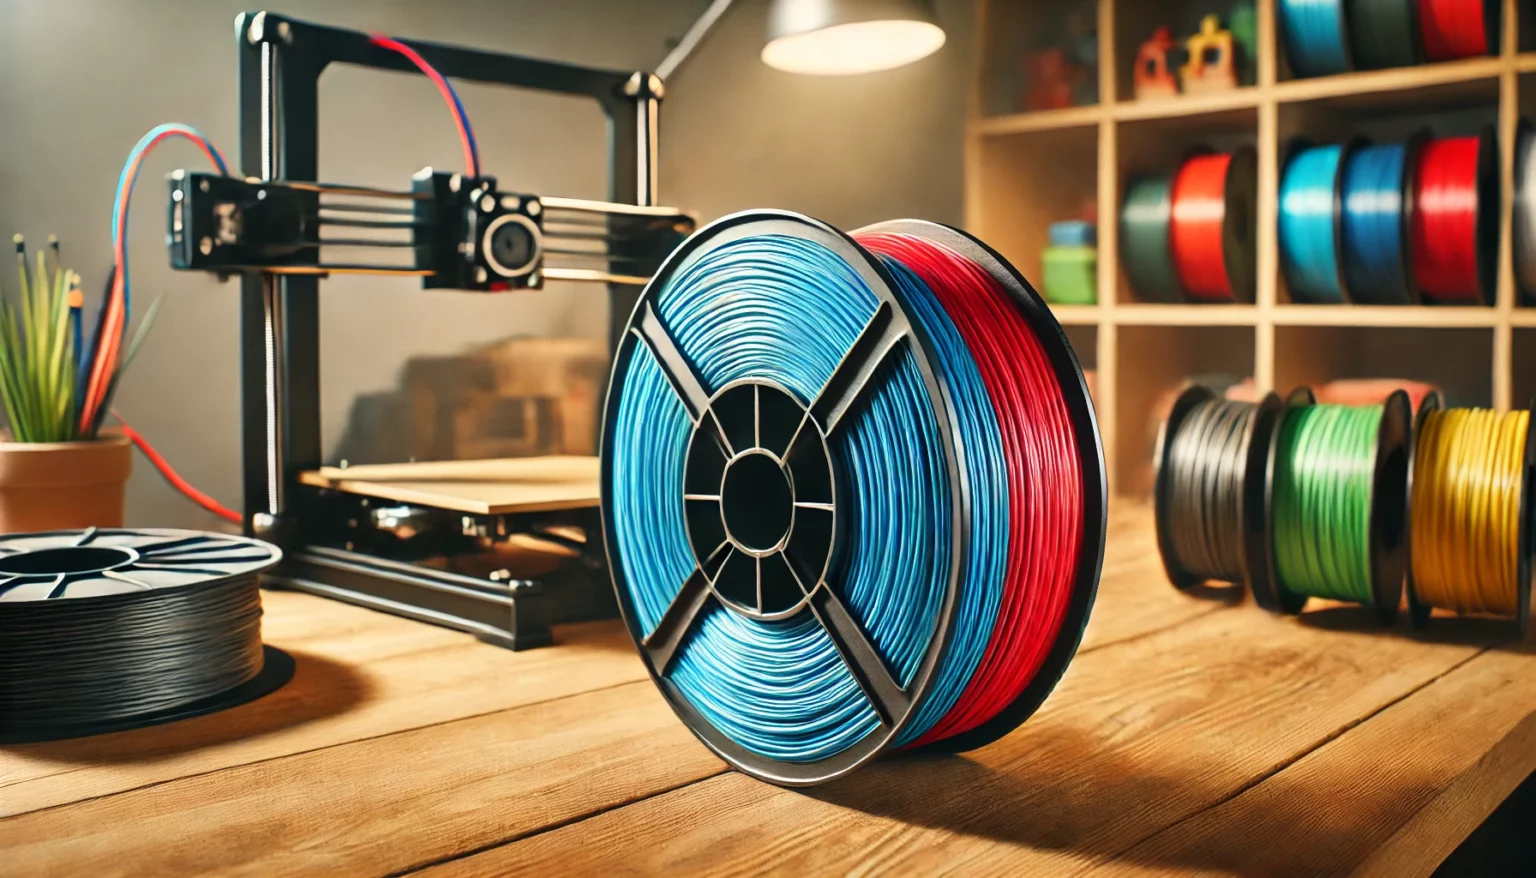
\includegraphics[width=0.4\textwidth]{components/image/pla_product.png}
    \caption{PLA filament for 3D printing \cite{pla_3d2print}.}
    \label{fig:pla_product}
\end{figure}

PLA is also environmentally friendly, as it is made from renewable resources and can be composted under the right conditions, unlike other petroleum-based materials like ABS. However, it has lower heat resistance and mechanical strength compared to its counterparts. 

PLA is suitable for a wide range of applications, including prototyping, educational projects, and hobbyist creations and thus is an excellent choice for the project due to its affordability, ease of printing and sufficient mechanical properties for the intended application.